\\[0.1in]
\begin{enumerate}
    \item[1و2.] هردو بخش اول این سوال را با هم حل می‌نماییم.
    ابتدا نشان می‌دهیم اگر هر مجموعه‌ای از 
    $A_n\;(n=1,2,3,\ldots)$
    شمارا و نامتناهی باشند، آنگاه 
    $\cup_{i=1}^\infty A_i$
    نیز شماراست. داریم:\\[0.15in]
    \begin{center}
        \begin{latin}
            For each $i\in \mathbb{N}$, choose a bijection $\phi_i:
            \mathbb{N} \longrightarrow A_i$, i.e. an ordering of the elements
            of $A_i$.
        \end{latin}
    \end{center}
    داریم:\newline
    \begin{center}
        \begin{latin}
            $a_{ij} = \phi_i(j) \xrightarrow{} a_{ij}$ is the j-th element of $A_i$
        \end{latin}
    \end{center}
    جدول زیر را در نظر بگیرید:\newline
    \begin{figure} [H]
        \centering
        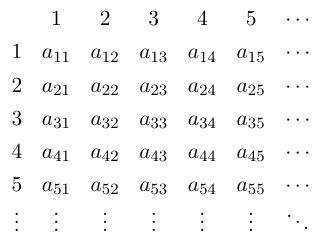
\includegraphics[scale=1]{solution/tab.png}
    \end{figure}
    به صورت زیگ-زاگی داریم:\newline
    \begin{center}
        $a_{11},a_{21},a_{12},a_{31},a_{22},a_{13}, \ldots$
    \end{center}
    بدین شکل یک bijection داریم که:\\[0.1in]
    \begin{center}
        $\phi : A \xrightarrow{} \mathbb{N}$\\[0.07in]
        $\longrightarrow a_{11} \mapsto 1,\; a_{21} \mapsto 2, \; \ldots$
    \end{center}
    پس نتیجه می‌گیریم که این ست شمارا می‌باشد.\newline
    حال در نظر بگیرید دو ست شمارا و نامتناهی $A$و $T$ را داشته باشیم. می‌خواهیم اثبات کنیم که
    $A\times T$ نیز شمارا می‌باشد.
    \begin{center}
        $(a, t)\in A\times T,\;\; a\in A, \;t\in T$
    \end{center}
    اگر تمامی عناصر $T$ را به شکل زیر لیست کنیم
    (چون می‌دانیم شمارا می‌باشد)،
    \begin{center}
        $t_1,t_2,t_3,\ldots$
    \end{center}
    آنگاه تمامی زیرمجموعه‌هایی در $A\times T$ که شامل زوج $(a,t_i)$ را $A_i$ بنامیم، آنگاه 
    $A_i$ شمارا خواهد بود از آنجا که یک bijection داریم:\newline
    \begin{center}
        $A\;\longrightarrow\;A_i \;\text{that maps}\; a\mapsto(a, t_i)$\\[0.1in]
        $A\times T = \bigcup_{i=1}^\infty A_i$
    \end{center}
    که به کمک بخش قبل ثابت می‌شود $A\times T$ شمارا می‌باشد.\\[0.1in]
    حالا در نظر بگیرید در همین بخش داشته باشیم $A=T$.
    در نتیجه طبق بخش قبل می‌دانیم $A\times A = A^2$ شماراست.
    حال در نظر بگیرید $T=A^2$. بنابراین $A\times A\times A = A^3$ شماراست. در نتیجه با استقرا روی $n$ نتیجه می‌گیریم که $A^n$ نیز شمارا می‌باشد. بنابراین طبق بخش اول،
    $\cup_{n=1}^\infty A^n$ هم باید شمارا باشد.\\[0.15in]
    در نتیجه هر دو خواسته بخش 1 و 2 را اثبات نمودیم.\newline
    \begin{eqnarray*}
        A^n \; &\sim& A \\[0.1in]
        \bigcup_{n=1}^\infty A^n \; &\sim& A
    \end{eqnarray*}
    \item[3.]
    این بخش را به طور مفصل توضیح می‌دهیم. چند نکته را دکر می‌نماییم و به اثبات کوناه آن‌ها می‌پردازیم.\\[0.2in]
    \begin{itemize}
        \item 
        برای اثبات و جزئیات بیشتر آن می‌توانید به 
        \href{https://web.williams.edu/Mathematics/lg5/CanBer.pdf}{اینجا}
        مراجعه کنید.
        \begin{figure} [H]
        \centering
        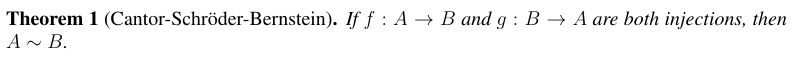
\includegraphics[scale=0.85]{solution/6-3-1.png}
        \end{figure}
        \item 
        داریم:
        \begin{center}
            $S=[0,1) \Longrightarrow \mathbb{R} \sim S$\\[0.1in]
        \end{center}
        برای مثال تابع 
        $\tan(x\pi+1)$
        ورودی آن بازه $S$ و خروجی آن $R$ می‌باشد و تناظر یک به یکی ایجاد می‌کند.
        \begin{figure} [H]
        \centering
        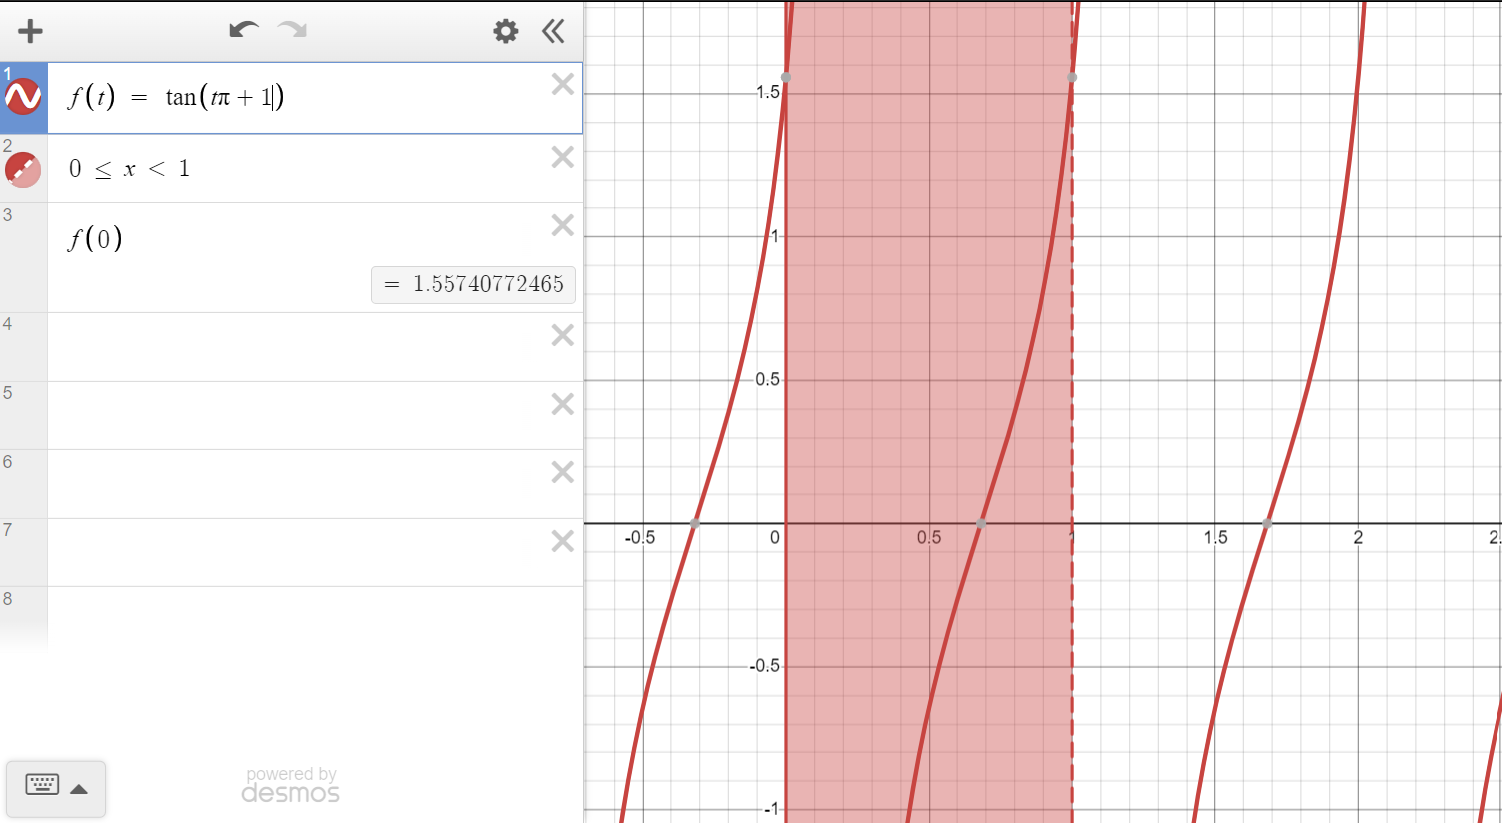
\includegraphics[scale=0.47]{solution/6-3-2.png}
        \end{figure}
        \item 
        داریم:
        \begin{center}
            $R\sim R^+,\;\;R\sim R^-$\\[0.1in]
        \end{center}
        توابع 
        $log(x)$ و $log(-x)$
        برای اثبات این بخش به کار می‌روند.
        \\[0.1in]
        \item 
        داریم:
        \begin{center}
            $S=[0,1) \Longrightarrow S^2 \sim S$\\[0.1in]
        \end{center}
        برای اثبات و جزئیات بیشتر آن می‌توانید به 
        \href{https://math.stackexchange.com/questions/183361/examples-of-bijective-map-from-mathbbr3-rightarrow-mathbbr/183383#183383}{اینجا}
        مراجعه کنید.\newline \newline
    \end{itemize}
    حال از نکات بالا استفاده می‌نماییم. داریم:
        \begin{eqnarray*}
            S = [0, 1) &\sim& \mathbb{R}\\
            A &\sim& \mathbb{R}\\
            \xrightarrow{second\; hint} 
            A &\sim& S\\
            \xrightarrow{S^2\sim S} A^2 &\sim& S\\
            &\vdots& induction\\
            A^n &\sim& S\\
            \xrightarrow{second\; hint} A^n &\sim& R\\
            \xrightarrow{Cantor-Schroder-Bernstein} A^n &\sim&
            A
        \end{eqnarray*}
        بنابراین بخش اول اثبات شد. برای بخش دوم داریم:\\[0.1in]
        \begin{eqnarray*}
            A &\sim& \mathbb{R}\\
            A^n &\sim& \mathbb{R}\\
            S_1=[0,1)&,&\;S_2=[1,2)\;\ldots\\
            A^n \sim S_n&,&\; A^{n-1} \sim S_{n-1}, \ldots\\
            \xrightarrow{} \bigcup_{n=1}^\infty A^n &\sim&
            \mathbb{R}^+\\
            \xrightarrow{\mathbb{R}^+ \sim \mathbb{R}}
            \bigcup_{n=1}^\infty A^n &\sim&
            \mathbb{R}
        \end{eqnarray*}
        و در نهایت به کمک
        \lr{Cantor-Schroder-Bernstein} ثابت می‌شود که:\\[0.1in]
        \begin{center}
            $\bigcup_{n=1}^\infty A^n \sim
            A$\\[0.2in]
        \end{center}
        برای اثبات این بخش، از لینک‌های زیر کمک گرفته شده است و اثبات‌های بیشتر و دقیق‌تر برای نکته‌های بیان شده، در آ‌ن‌ها آمده است.
        \begin{itemize}
            \item 
                \href{https://math.stackexchange.com/questions/1071261/how-the-cardinality-of-mathbbr-and-mathbbr-same#:~:text=Logarithmic%20map%20is%20from%20R,R%2B%20and%20R%20is%20same.}{لینک اول}
            \item 
                \href{https://math.stackexchange.com/questions/183361/examples-of-bijective-map-from-mathbbr3-rightarrow-mathbbr/183383#183383}{لینک دوم}
            \item 
                \href{https://math.stackexchange.com/questions/290019/cardinality-of-mathbbr-and-mathbbr2}{لینک سوم}
            \item 
                \href{https://web.williams.edu/Mathematics/lg5/CanBer.pdf}{لینک چهارم}
            \item 
                \href{https://web.uvic.ca/~gmacgill/LFNotes/Cardinality.pdf}{لینک پنجم}
        \end{itemize}
\end{enumerate}